\documentclass[a4paper, 11pt]{article}
\usepackage{amsmath}
\usepackage{graphicx}
\usepackage{geometry}
\usepackage{listings}
\usepackage[colorlinks,linkcolor=red]{hyperref}
\geometry{scale=0.8}

\title{	
\normalfont \normalsize
\textsc{School of Data and Computer Science, Sun Yat-sen University} \\ [25pt] %textsc small capital letters
\rule{\textwidth}{0.5pt} \\[0.4cm] % Thin top horizontal rule
\huge  Maze Problem\\ % The assignment title
\rule{\textwidth}{2pt} \\[0.5cm] % Thick bottom horizontal rule
\author{16337102 HuangZi lin}
\date{\normalsize\today}
}

\begin{document}
\maketitle
\tableofcontents
\newpage
\section{Task}



\begin{itemize}
	\item Please solve the maze problem by using BFS or DFS (Python or C++)
	\item The maze layout can be modeled as an array, and you can use the data file \texttt{MazeData.txt} if necessary.
	\item Please send \texttt{E01\_YourNumber.pdf} to \texttt{ai\_2018@foxmail.com}, you can certainly use \texttt{E01\_Maze.tex} as the \LaTeX template.
\end{itemize}

\begin{figure}[ht]
\centering
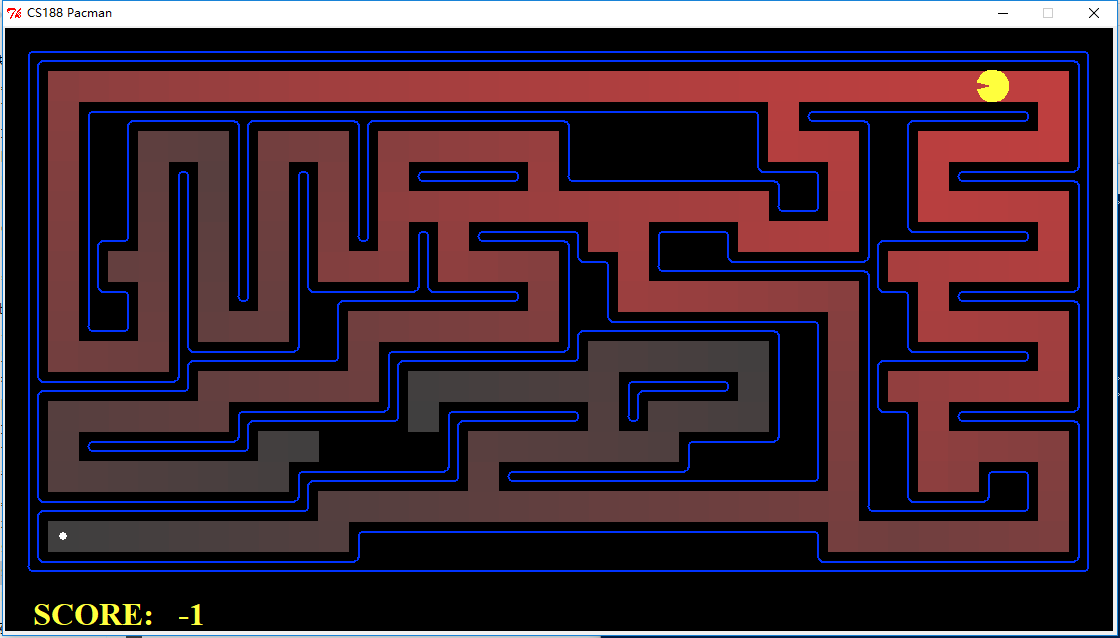
\includegraphics[width=15cm]{Pic/Pacman}

\caption{Searching by BFS or DFS}
\end{figure}
\section{Codes}
\lstset{language=Python}
%%\lstset{language=Python}
\begin{lstlisting}
import numpy as np

f = open("MazeData.txt", 'r')
data = []
for i in range(18):
    data.append(f.readline())
datas = []
for i in data:
    for n in i:
        if n != '\n':
            datas.append(n)
f.close()

data = [[0 for i in range(36)] for j in range(18)]
for i in range(18):
    for n in range(36):
        data[i][n] = datas[36 * i + n]

n = 0
start_x = 0
start_y = 0
end_x = 0
end_y = 0

for i in range(18):
    for n in range(36):
        if data[i][n] == 'S':
            start_x = i
            start_y = n
        elif data[i][n] == 'E':
            end_x = i
            end_y = n

path = []
if start_x >= end_x and start_y >= end_y:
    move = np.array([[-1, 0], [0, -1], [1, 0], [0, 1]])
elif start_x >= end_x and start_y <= end_y:
    move = np.array([[-1, 0], [0, 1], [1, 0], [0, -1]])
elif start_x <= end_x and start_y >= end_y:
    move = np.array([[1, 0], [0, -1], [-1, 0], [0, 1]])
else:
    move = np.array([[1, 0], [0, 1], [-1, 0], [0, -1]])

def inPath(x, y, path):
    if [x, y] in path:
        return True
    else:
        return False

def run(start_x, start_y, end_x, end_y, move):
    if start_x == end_x and start_y == end_y:
        return
    elif data[start_x + move[0][0]][start_y+move[0][1]] != '%' 
                and not inPath(start_x + move[0][0], start_y + move[0][1], path):
        if start_x == end_x and start_y == end_y:
            return
        start_x += move[0][0]
        start_y += move[0][1]
        path.append([start_x, start_y])
        run(start_x, start_y, end_x, end_y, move)
        start_x -= move[0][0]
        start_y -= move[0][1]
    elif data[start_x + move[1][0]][start_y + move[1][1]] != '%' 
                and not inPath(start_x + move[1][0], start_y + move[1][1], path):
        if start_x == end_x and start_y == end_y:
            return
        start_x += move[1][0]
        start_y += move[1][1]
        path.append([start_x, start_y])
        run(start_x, start_y, end_x, end_y, move)
        start_x -= move[1][0]
        start_y -= move[1][1]
    elif data[start_x + move[2][0]][start_y + move[2][1]] != '%' 
                and not inPath(start_x + move[2][0], start_y + move[2][1], path):
        if start_x == end_x and start_y == end_y:
            return
        start_x += move[2][0]
        start_y += move[2][1]
        path.append([start_x, start_y])
        run(start_x, start_y, end_x, end_y, move)
        start_x -= move[2][0]
        start_y -= move[2][1]
    elif data[start_x + move[3][0]][start_y + move[3][1]] != '%' 
                and not inPath(start_x + move[3][0], start_y + move[3][1], path):
        if start_x == end_x and start_y == end_y:
            return
        start_x += move[3][0]
        start_y += move[3][1]
        path.append([start_x, start_y])
        run(start_x, start_y, end_x, end_y, move)
        start_x -= move[3][0]
        start_y -= move[3][1]
    else:
        path.pop()
        return

run(start_x, start_y, end_x, end_y, move)
print(path)
print(start_x, start_y)
print(end_x, end_y)
for i in path:
    data[i[0]][i[1]] = '*'

doc = open('out.txt', 'w')
for i in range(18):
    for n in range(36):
        print(data[i][n], end = '', file=doc)
    print('', file=doc)
doc.close()
\end{lstlisting}


\section{Results}
\begin{figure}
\centering
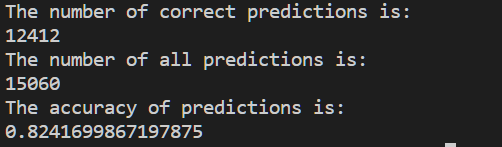
\includegraphics[width=15cm]{result.png}
\end{figure}


%\clearpage
%\bibliography{E:/Papers/LiuLab}
%\bibliographystyle{apalike}
\end{document}
